\documentclass[9pt,a4paper]{extarticle}
\usepackage[margin=1.25cm,top=1.1cm,bottom=1.0cm]{geometry}
\usepackage{fontspec}
\setmainfont{Apple SD Gothic Neo}
\setmonofont{Menlo}[Scale=0.82]
\usepackage{graphicx,booktabs,xcolor,enumitem,titlesec,array}
\XeTeXlinebreaklocale "ko"
\XeTeXlinebreakskip=0pt plus 1pt
\setlength{\parindent}{0pt}\setlength{\parskip}{2.5pt}
\pagestyle{empty}
\titleformat{\section}{\normalsize\bfseries\color[HTML]{B3261E}}{}{0pt}{}
\titlespacing{\section}{0pt}{5pt}{2pt}
\setlist{nosep,leftmargin=1.2em}
\newcommand{\col}[1]{\texttt{#1}}
\begin{document}
{\Large\bfseries 합정역 버스 데이터 기록 점검}\hfill 2026-11-12, 브랜치 \col{feat/hapjeong-road-audit-and-data}

\vspace{2pt}\hrule\vspace{4pt}
\textbf{결론.} 합정역에서 버스 ego로 수집이 돌고, 수업 필수 컬럼 19개와 팀 추가 7개가 모든 행에 있다.
버스 제원과 jerk도 기록된다. 다만 규칙으로 달린 버스는 다른 차와 거의 마주치지 않아, 지금 데이터는 상호작용 데이터로 쓰기 어렵다.

\section{수집한 것}
\begin{tabular}{@{}>{\raggedright}p{3.1cm}p{14.6cm}@{}}
조건 & 지도 \col{hapjeong} 3.0.0, 경로 \col{bus\_loop}(1,988m), 교통량 busy, 경로 추종 규칙, seed 0\textasciitilde 7 \\
결과 & 8에피소드 4,889스텝. 8개 모두 도착으로 끝났다. 8개 병렬로 21초(초당 232스텝) \\
$10^7$개 추정 & 같은 속도면 약 12시간. 한 번 잰 값이고 SUMO 시작과 예열 180초를 포함한다 \\
검사 & \col{scripts/export\_csv.py}가 모든 행의 컬럼, \col{state} 안쪽 키, 가속 한계를 검사한 뒤에만 CSV를 쓴다 \\
\end{tabular}

\section{컬럼 26개}
\begin{tabular}{@{}>{\raggedright}p{3.1cm}p{14.6cm}@{}}
\toprule
수업 필수 19개 & \col{episode}, \col{t}, \col{observation}(31차원), \col{action\_raw}, \col{action.*} 4개, \col{reward}, \col{terminated}, \col{truncated}, \col{state}, \col{detected\_vehicles}, \col{event.*} 4개, \col{next\_observation}, \col{next\_state} \\
팀 추가 7개 & \col{sim\_time}, \col{detected\_pedestrians}, \col{event.termination\_reason}, \col{comfort.peak\_acceleration}, \col{comfort.peak\_jerk}, \col{comfort.acceleration\_violation}, \col{comfort.jerk\_violation} \\
\col{state} 안쪽 & \col{ego}(위치, 속도, 가속도, jerk, 차로, 방향지시등), \col{vehicles}와 \col{pedestrians}(ego에서 150m 안), \col{navigation}(다음 회전, 횡단보도, 정류장까지 거리), \col{traffic\_light}(상태, 정지선까지 거리) \\
감지 목록 & \col{detected\_vehicles}는 관측 차선의 차량과 50m 안의 차량이다. ego 차체 좌표의 상대 위치, 상대 속도, 방향지시등을 적는다. 보행자는 50m 안 \\
\bottomrule
\end{tabular}

\section{버스 특성이 데이터에 남는가}
\begin{tabular}{@{}>{\raggedright}p{3.1cm}>{\raggedright}p{6.0cm}p{8.3cm}@{}}
\toprule
10/29 회의의 버스 특징 & 기록되는 곳 & 확인한 값 \\
\midrule
긴 차체 & metadata의 \col{ego} (길이 12m, 폭 2.5m) & SUMO 차량 타입에 그대로 들어간다 \\
제한된 가속 & \col{state.ego.acceleration} & 4,889스텝에서 $-2.0$\textasciitilde$+1.0$ m/s². 제원 한계와 같다 \\
승객 편안함 & \col{state.ego.jerk}, \col{comfort.*} & jerk 한계(2.0 m/s³) 위반 188스텝(3.8\%) \\
정류장 & \col{state.navigation.distance\_to\_stop} & 거리만 기록한다. 버스는 정류장에 서지 않는다 \\
승객 승하차, 버스 간 거리, 정류장 점유 & 없음 & 구현하지 않았다. 설계안에서 연구용 항목은 빼기로 했다 \\
\bottomrule
\end{tabular}

\vspace{3pt}
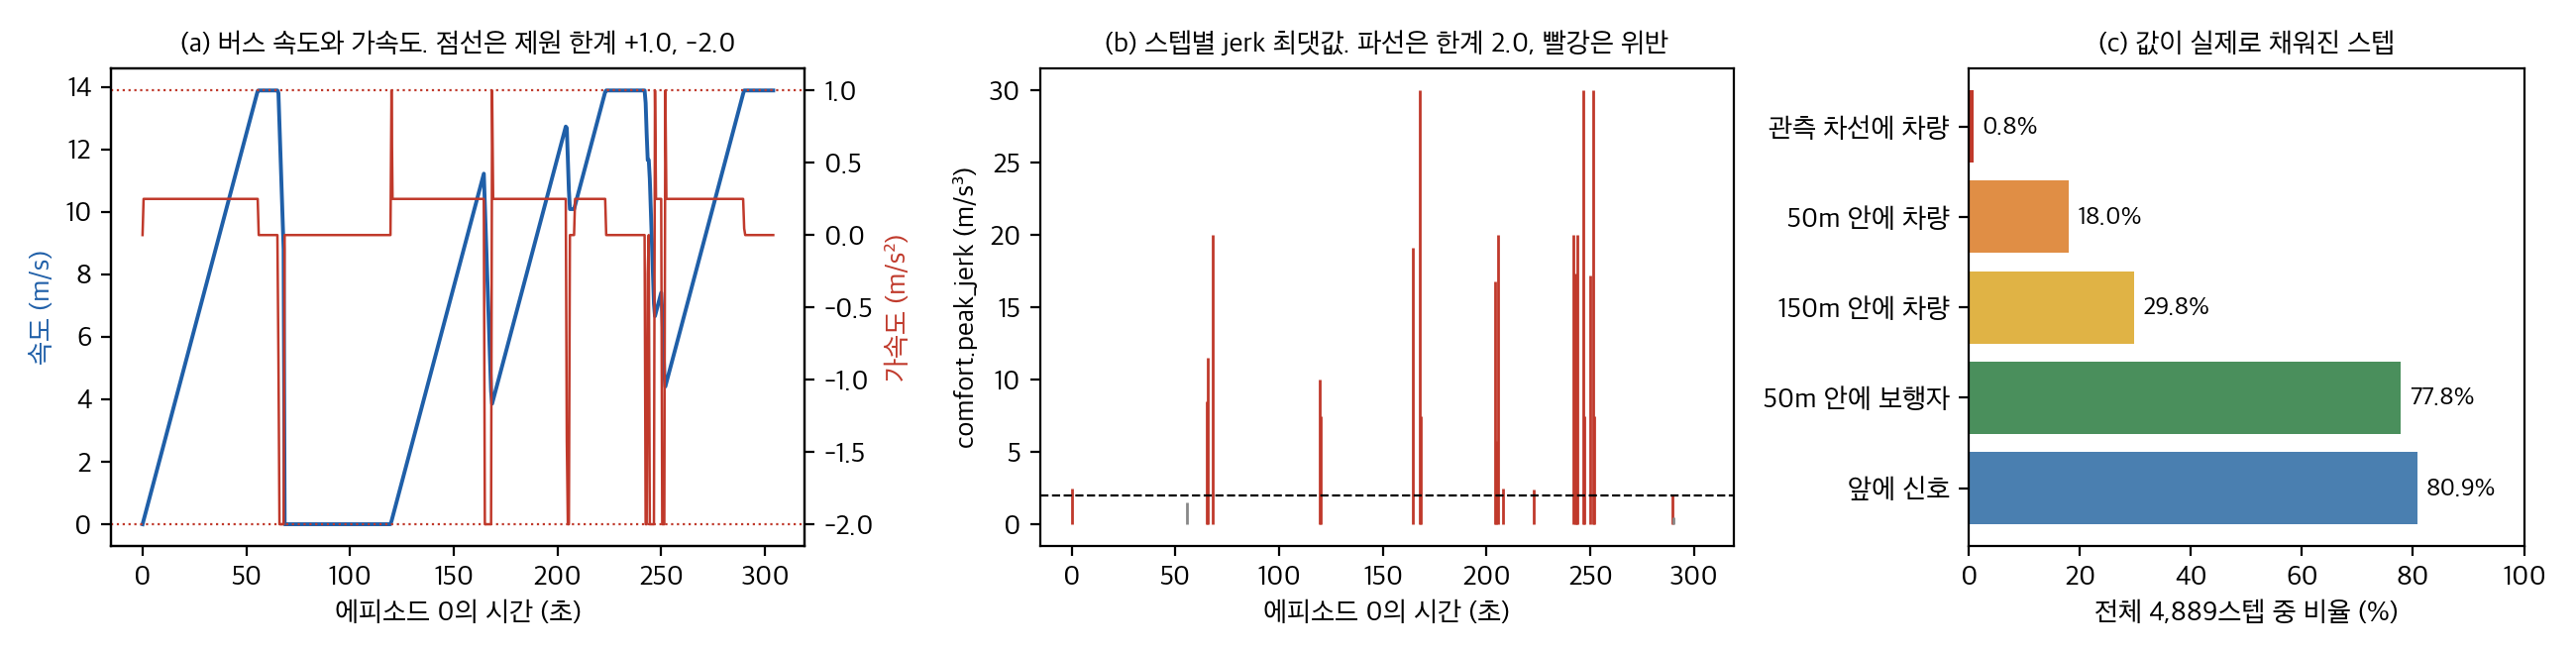
\includegraphics[width=\linewidth]{figure.png}

\section{수집하면서 고친 것}
\begin{itemize}
\item \textbf{ego가 승용차였다.} \col{main}의 ego는 가속 5.4 m/s²의 승용차였다. 10월에 정한 버스 제원을 넣고 \col{map.json}의 \col{ego\_vehicle}이 고르게 했다.
\item \textbf{jerk가 행동과 무관하게 튀었다.} 환경이 목표 속도를 0.5초마다 한 번에 줘서, 첫 0.1초에 최대 가속으로 따라붙고 나머지는 등속이었다. 1,210스텝 중 786스텝이 한계를 넘었다. 가속도를 0.5초 내내 고르게 적용하자 1,218스텝 중 48스텝이 됐다. 남은 위반은 SUMO 안전 보조가 신호 앞에서 제동을 시작하는 순간이 대부분이다.
\item \textbf{합정역에서 환경이 돌지 않았다.} 0번 차로가 인도라 막혀 있었다. 환경이 버스가 다닐 수 없는 차로를 없는 차로로 보게 했다.
\item \textbf{교차로 안에서 경로 거리가 최대 12m 어긋났다.} 독립 리뷰가 찾았다. 고친 뒤 4,889스텝에서 거리 역행은 0건이다.
\end{itemize}

\section{설계안과 다른 점, 회의에서 정할 것}
\begin{itemize}
\item \textbf{상호작용이 드물다.} 그림 (c)처럼 관측 차선에 차가 있던 스텝은 0.8\%다. 규칙 버스의 주행 시간은 교통량과 seed에 관계없이 9회 모두 304.5초였다. 버스 접근에 맞춰 차를 넣는 장치(주현진)와 학습된 정책이 있어야 한다.
\item \textbf{관측은 31차원 그대로다.} 설계안의 새 관측 구성(보행자, 신호, 방향지시등 입력)은 만들지 않았다. 그 정보는 \col{state}와 감지 목록에만 있다.
\item \textbf{jerk 한계의 정의.} 지금은 0.1초 간격의 가속도 차이라, 가속 명령이 0.2 m/s² 넘게 바뀌면 위반이다. 0.5초 단위로 잴지, 한계값을 바꿀지 정해야 한다.
\item \textbf{제출 파일.} \col{data/submission/} 폴더의 00조\_칼럼설명.pptx와 00조\_데이터예시.csv(15행). 조 번호를 바꾸고 zip으로 묶으면 된다.
\end{itemize}
\end{document}
